\chapter{Simulation und Testplanung}
Um das Potentialfeld auch ohne Robotinos zu testen, wird zu Beginn des Projektes mit einer vereinfachten Simulation das Potentialfeld auf Ihre Funktionsfähigkeit geprüft. Bei dieser Simulation wird der Robotino als enfache I-Strecke betrachtet. Dabei wird der Ausgang der Strecke auf den Istpositionsinput gegeben und der berechnete Geschwindigkeitsvektor auf die Strecke gegeben. Desweiteren werden auf die restlichen Inputs Konstanten gegeben und die Ausgangsdaten in einer Logdatei abgespeichert. Da nach wenigen Versuchen erkennbar ist, dass das Potentialfeld seine Funktion erfüllt, wird im folgenden mit dem Robotinos direkt getestet. Dazu wird zu Beginn der Fertigungsbereich nicht betrachtet und nur ein Festprogrammiertes Ziel angefahren. Um flexibel Ziele anfahren zu können und die Schnittstelle mit der Fertigungsplanung zu teseten wird ein UDP-Dummy in Simulink erstellt mit dem Aufträge an den Robotino per UDP in Simulink gesendet werden können. Dadurch können mehrere Ziele hintereinander Angefahren werden. Im nächsten Schritt wird die Schnittstelle mit der Bahnregelung gestestet dazu werden beide Simulinkmodelle kombiniert und auf den Robotino geladen. Dadurch können Schnittstellenprobleme zwischen der Bahnregeleung und der Bahnplanung frühzeitig behoben werden. Da sich im laufe des Projektes gezeigt hat, dass die Fertigungsplanung den Gesamtsystemtesttermin nicht einhalten kann, wird der UDP-Dummy in zusammenarbeit mit der Bahnregelung dahingehend erweitert, zufallsgenerierte Aufträge zu senden. Im letzten Schritt wird der UDP-Dummy als Fertigungsplanungsersatz erweitert indem sich die Positionen der Werkstücke gemerkt wird und die zufallsgenerierten Aufträge auf ausführbare Aufträge gefiltert wird. Zum Ende des Projektes wird zusätzlich eine Simulation, wie zu Beginn, mit der Erweiterung auf 5 Robotinos ausgeführt um geringe Änderungen im Programm aufzuzeichnen, da die Aufzeichnung von Daten von mehreren Robotinos unter Simulinkrealtime einige Probleme verursacht. Unter Kapitel \ref{} wird eine Simulation des Ausweichmanövers dargestellt.
\section{Simulation des Ausweichmanövers}
In diesem Abschnitt wird die Simulation des Ausweichmanövers dargestellt. Dazu werden zwei Simulationen miteinander Verglichen. In der ersten Simulation, welche in Abbildung \ref{fig:SimulationAusweich} dargestellt ist, werden zwei Robotinos betrachtet. Robotino 1 in Rot dargestellt fährt von der Position [500 1000] zur Station 7 welche sich ganz rechts befindet. Robotino 2 in blau dargestellt fährt von der Position [4500 1000] zur Station 0 welche sich ganz links befindet. Wie in der Abbildung zu sehen ist, umfahren sich die Robotinos rechts herum.

\begin{figure}
	\centering	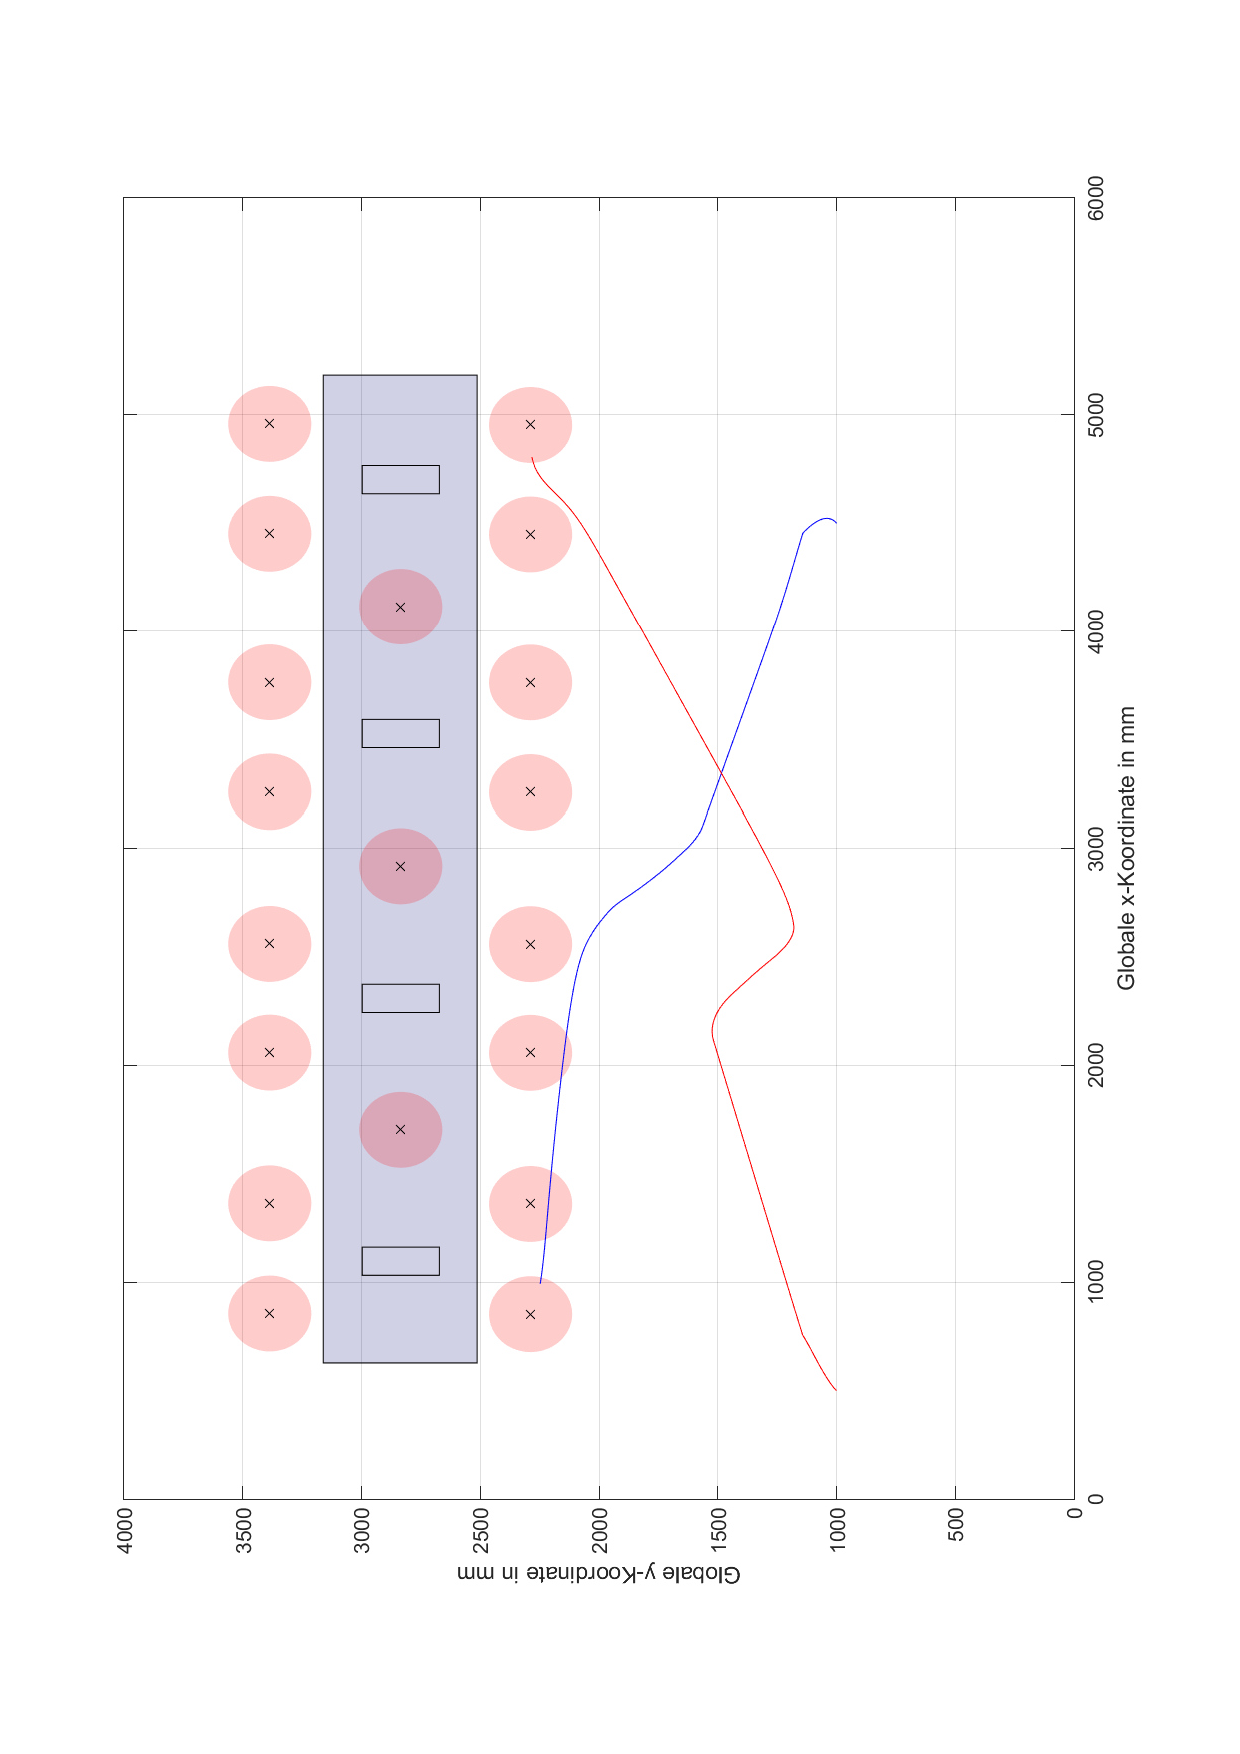
\includegraphics[width=0.5\textwidth,angle=-90]{grafiken/SimulationAusweich.pdf}
	\caption{Simulation mit Ausweichfunktion}
	\label{fig:SimulationAusweich}
\end{figure}

 In der zweiten Simulation, welche in Abbildung \ref{fig:SimulationohneAusweich} dargestellt ist, werden die gleichen Robotinos mit der gleichen Start und Zielposition betrachtet. In dieser Simulation wird jedeglich die Ausweichfunktion auf Null gesetzt. Wie in der Abbildung zu erkennen ist, kommt es zu einem Abstoßverhalten, wodurch die Robotinos stark ausgebremst werden. Wie in den Abbildungen zu erkennen ist, hat die entwickelte Ausweichfunktion eine Verbesserung im Ausweichverhalten verursacht.
 
\begin{figure}
	\centering	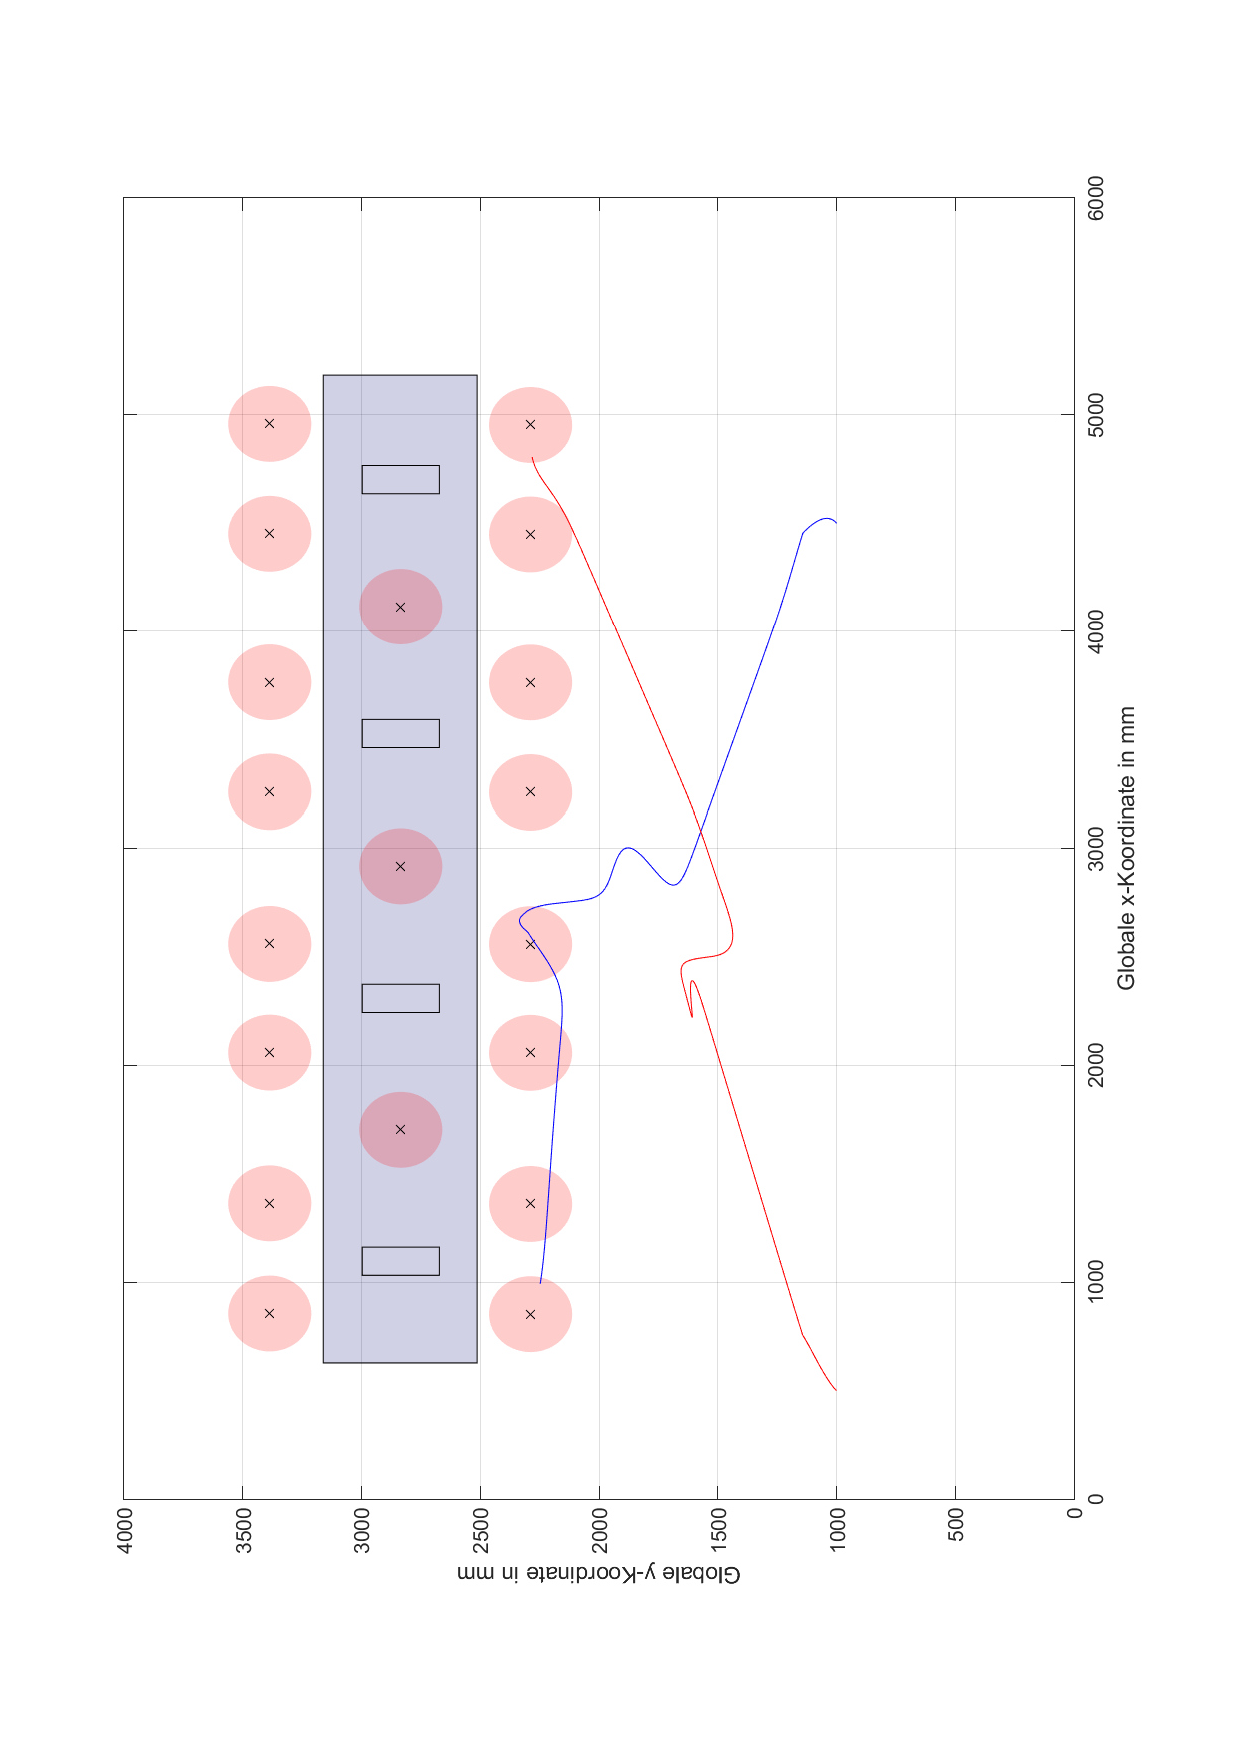
\includegraphics[width=0.5\textwidth,angle=-90]{grafiken/Simulation_ohne_Ausweich}
	\caption{Simulation ohne Ausweichfunktion}
	\label{fig:SimulationohneAusweich}
\end{figure}
\section{Simulation Wartebereiche}